\chapter{ปัญหาวิถีสั้นสุด (Shortest Path Problem)}

ปัญหา Shortest path คือปัญหาที่ต้องการหาทางเดินสั้นที่สุดระหว่าง 2 จุดยอดภายในกราฟ ตัวอย่างปัญหานี้สามารถพบได้ทั่วไปในชีวิตประจำวัน เช่น การหาวิธีเดินทางจากเมืองหนึ่งไปยังอีกเมืองหนึ่งในแผนที่ โดยกำหนดให้จุดยอดแทนเมืองต่างๆ และเส้นเชื่อมแทนด้วยถนนหรือเส้นทาง และนำ้หนักของเส้นเชื่อมแทนด้วยเวลาที่ใช้ในการเดินทางบนเส้นทางนั้นๆ

ปัญหาวิถีสั้นสุด สามารถแบบออกได้เป็น 2 รูปแบบหลักๆ
\begin{enumerate}
\item ปัญหาวิธีสั้นสุดแบบแหล่งต้นทาง/ปลายทางเดียว (Single Source Shortest Path Problem)
\item ปัญหาวิธีสั้นสุดแบบทุกคู่จุด (All Pairs Shortest Path Problem)
\end{enumerate}

\section{ปัญหาวิธีสั้นสุดแบบแหล่งต้นทาง/ปลายทางเดียว (Single Source Shortest Path Problem : SSSP)}

ปัญหารูปแบบนี้จะมีการกำหนดแหล่งต้นทางหรือแหล่งปลายทาง อย่างน้อย 1 แหล่งมาให้ เรียกว่าจุดยอด $u$  สิ่งที่ต้องการทราบ คือ วิถีสั้นสุดจากจุดยอด $u$ ไปยังจุดยอดใดๆ ภายในกราฟ

มีหลายขั้นตอนวิธีที่สามารถใช้แก้ปัญหานี้ได้ แต่ละวิธีก็มีข้อดีและข้อเสียแตกต่างกันออกไป ในด้าน Space/Time complexity

\subsection{ขั้นตอนวิธีของเบลแมน-ฟอร์ด (Bellman-Ford Algorithm)}

Bellman-Ford algorithm นอกจากจะสามารถใช้แก้ปัญหา SSSP ได้แล้วยังมีความพิเศษอีกหนึ่งอย่าง คือ สามารถตรวจพบวัฏจักรเชิงลบ (Negative cycle) ได้อีกด้วย

\newpage

\begin{lstlisting}
struct edge {
	int u, v, w;
};
int bellman_ford(int n, int st, int en, vector<edge> edges){
	int dis[n];
	dis[st] = 0;
	for (int i = 1; i < n; i++){
		for (auto x : edges){
			if (dis[x.u] + x.w < dis[x.v])
				dis[x.v] = dis[x.u] + x.w;
			if (dis[x.v] + x.w < dis[x.u])
				dis[x.u] = dis[x.v] + x.w;
		}
	}
	for (auto x : edges){
		if (dis[x.u] + x.w < dis[x.v] || dis[x.v] + x.w < dis[x.u])
			return -1; // Negative weight cycle detected
	}
	return dis[en];
}
\end{lstlisting}

\begin{figure}[h!]
	\centering
    \begin{subfigure}{.5\textwidth}
    	\centering
    	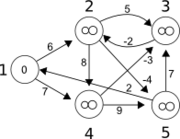
\includegraphics[width=4cm]{images/bellman-ford-1}
    	\caption{กราฟที่ระบุระยะทางที่สั้นที่สุดจากจุดยอด 1 ไปยังจุดยอดทั้งหมด}
    	\label{fig:bellman_ford_1}
    \end{subfigure}%
    \begin{subfigure}{.5\textwidth}
    	\centering
    	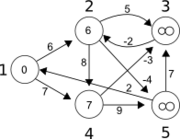
\includegraphics[width=4cm]{images/bellman-ford-2}
    	\caption{ผลลัพธ์หลังการทำงานรอบที่ 1}
    	\label{fig:bellman_ford_2}
    \end{subfigure}
     \begin{subfigure}{.5\textwidth}
    	\centering
    	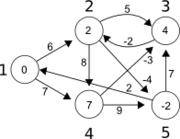
\includegraphics[width=4cm]{images/bellman-ford-final}
    	\caption{ผลลัพธ์หลังการทำงาน $n-1$ รอบ}
    	\label{fig:bellman_ford_2}
    \end{subfigure}
    \caption{ตัวอย่างขั้นตอนวิธีของเบลแมน-ฟอร์ด}
    \label{fig:bellman_ford_example}
\end{figure}

หลักการทำงาน จะเริ่มต้นพิจารณาจากแนวคิดพื้นฐานว่าเส้นทางที่สั้นที่สุดไปยังจุดยอดทั้งหมดเป็นอนันต์ ยกเว้นระยะทางไปยังแหล่งต้นทางที่มีระยะทางเป็น 0

จากนั้น จึงพิจารณาทุกเส้นเชื่อมในกราฟ หากเส้นเชื่อมใด ``ตึง'' ให้ลอง ``ผ่อน'' เส้นเชื่อมนั้น เริ่มแรกเมื่อตรวจสอบที่เส้นทางจากจุดยอด 1 ไปยังจุดยอด 2 พบว่ามีนำ้หนักเส้นเชื่อมคือ 6 ซึ่งมีค่าน้อยกว่าอนันต์ จึงแทนค่าอนันต์ในจุดยอด 2 ด้วย 6 และพิจารณาเส้นทางจากจุดยอด 1 ไปยังจุดยอด 4 พบว่าเส้นเชื่อมคือ 7 ซึ่งน้อยกว่าอนันต์ จึงแทนค่าอนันต์ในจุดยอดที่ 4 ด้วย 7

การพิจารณาทุกเส้นเชื่อมในกราฟครบ 1 รอบ จะสามารถรับประกันได้ว่าจะมีอย่างน้อย 1 จุดยอดที่มีเส้นทางที่สั้นที่สุดแล้ว จึงต้องทำการพิจารณาทุกเส้นเชื่อมให้ครบ $n-1$ รอบ เพื่อรับประกันทุกจุดยอดในกราฟ

\begin{question}
เพราะเหตุใดจึงสามารถพิจารณาแค่ $n-1$ รอบได้ ในเมื่อมีจุดยอดทั้งหมด $n$ จุด
\end{question}

วิธีการตรวจสอบวัฎจักรเชิงลบ สามารถทำได้โดยการทำการพิจารณาทุกเส้นเชื่อมในกราฟอีกหนึ่งรอบเป็นรอบที่ $n$ หากยังมีการเปลี่ยนแปลงของระยะทาง แสดงว่าเกิดวัฎจักรเชิงลบเกิดขึ้น

เวลาที่ใช้ในการทำงานของขั้นตอนวิธีนี้ คือ $O(|V||E|)$ เนื่องจากมีการทำงานทั้งหมด $n-1$ รอบ และแต่ละรอบมีการพิจารณาเส้นเชื่อมทุกเส้น

\subsection{ขั้นตอนวิธีของไดก์สตรา (Dijkstra's Algorithm)}

สำหรับขั้นตอนวิธีนี้จะหาระยะทางสั้นที่สุดจากจุดหนึ่งไปยังจุดใด ๆ ในกราฟโดยจะหาเส้นทางที่สั้นที่สุดไปทีละจุดยอดเรื่อย ๆ จนครบตามที่ต้องการ วิธีนี้มีข้อจำกัดสำหรับกราฟที่มีความยาวของเส้นเชื่อมไม่เป็นลบเท่านั้น

\begin{lstlisting}
struct node{
	int current_node, total_distance;
	node(int n, int d) : current_node(n), total_distance(d) {}
	bool operator<(const node &o) const{
		return total_distance > o.total_distance;
	}
};
int dijkstra(int N, int source, int destination, vector<pair<int, int>> g[]){
	int dis[N];
	priority_queue<node> heap;
	fill(dis, dis + N, 2e9);
	dis[source] = 0;
	heap.push({source, 0});
	while (!heap.empty()){
		auto now = heap.top();
		heap.pop();
		for (auto x : g[now.current_node]){
			if (dis[x.first] <= now.total_distance + x.second)
				continue;
			dis[x.first] = now.total_distance + x.second;
			heap.push({x.first, dis[x.first]});
		}
	}
	return dis[destination];
}
\end{lstlisting}


หลักการทำงานของขั้นตอนวิธีนี้ คือ
\begin{enumerate}
\item กำหนดให้ทุกจุดยอดมีค่าระยะทางเป็นอนันต์ ยกเว้นจุดยอดเริ่มต้นมีค่าเป็นศูนย์
\item นำจุดยอดเริ่มต้นใส่ลงไปในเซตของจุดยอดที่กำลังพิจารณา
\item จากจุดยอดปัจจุบัน พิจารณาจุดยอดข้างเคียงตามเส้นเชื่อมทุกจุด และคำนวณระยะทางต่อเนื่องของเส้นเชื่อมมาเปรียบเทียบกับระยะทางเดิมของจุดยอดนั้นๆ ตัวอย่างเช่น ถ้าจุดยอดปัจจุบันคือ $A$ มีระยะทางของจุดยอดเป็น 6 และเส้นเชื่อมที่ต่อจาก $A$ ไปยังจุดยอดข้างเคียง $B$ มีระยะทางเป็น 2 ดังนั้นระยะทางของจุดยอด $B$ (โดยผ่าน $A$) จึงเท่ากับ $6+2 = 8$ เป็นต้น ถ้าระยะทางที่คำนวณได้มีค่าน้อยกว่าค่าระยะทางที่บันทึกอยู่ของจุดยอดนั้น ให้เขียนทับค่าระยะทางดังกล่าว และนำจุดยอดนั้นเข้าเซตของจุดยอดที่กำลังพิจารณา
\item หลังจากพิจารณาจุดยอดข้างเคียงของจุดยอดปัจจุบันทั้งหมดแล้ว ให้นำจุดยอดปัจจุบันออกจากเซตของจุดยอดที่กำลังพิจารณา
\item จุดยอดถัดไปจะเป็นจุดยอดที่อยู่ในเซตของจุดยอดที่กำลังพิจารณาและมีต่าระยะทางน้อยที่สุด
\item วนกลับไปทำขั้นตอนที่ 3 จนกว่าเซตของจุดยอดที่กำลังพิจารณาจะหมด หรือพิจารณาจุดยอดปลายทางแล้ว
\end{enumerate}
$O(|V|+|E|log|V|)$

\section{ปัญหาวิธีสั้นสุดแบบทุกคู่จุด (All Pairs Shortest Path Problem : APSP)}
